\documentclass[class=article,border=5pt,tikz]{standalone}
\usetikzlibrary{calc}

\newcommand*{\nx}{5}
\newcommand*{\ny}{5}

\newcommand*{\ColorCells}[1]{% #1 = list of x/y/color
  \foreach \x/\y/\color in {#1} {
    \node [fill=\color, draw=none, thick, minimum size=1cm] 
      at (\x-.5,\ny+0.5-\y) {};
    }%
}%



\begin{document}

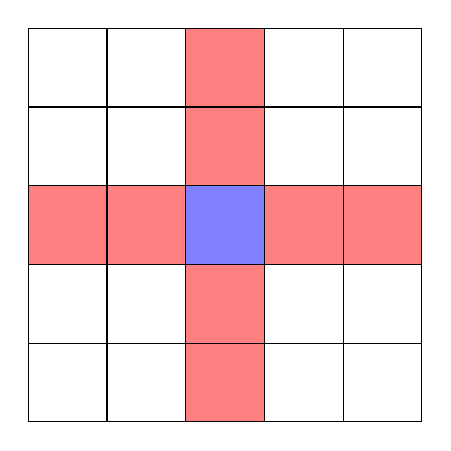
\begin{tikzpicture}
  \ColorCells{3/3/blue!50}
  \ColorCells{2/3/red!50, 1/3/red!50, 4/3/red!50, 5/3/red!50, 3/2/red!50, 3/1/red!50, 3/4/red!50, 3/5/red!50}
  \draw (0, 0) grid (\nx, \ny);
\end{tikzpicture}

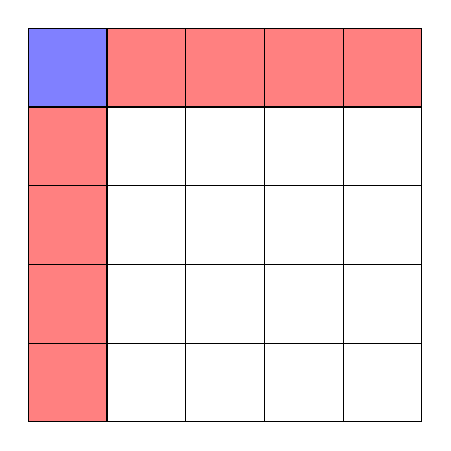
\begin{tikzpicture}
  \ColorCells{1/1/blue!50}
  \ColorCells{1/2/red!50, 1/3/red!50, 1/4/red!50, 1/5/red!50, 2/1/red!50, 3/1/red!50, 4/1/red!50, 5/1/red!50}
  \draw (0, 0) grid (\nx, \ny);
\end{tikzpicture}

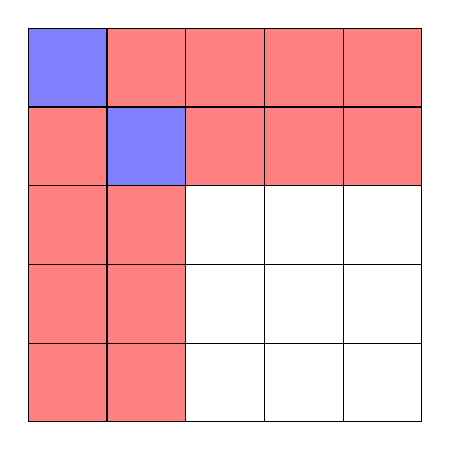
\begin{tikzpicture}
  \ColorCells{1/1/blue!50}
  \ColorCells{1/2/red!50, 1/3/red!50, 1/4/red!50, 1/5/red!50, 2/1/red!50, 3/1/red!50, 4/1/red!50, 5/1/red!50}
  \ColorCells{2/2/blue!50}
  \ColorCells{2/3/red!50, 2/4/red!50, 2/5/red!50, 3/2/red!50, 4/2/red!50, 5/2/red!50}
  \draw (0, 0) grid (\nx, \ny);
\end{tikzpicture}

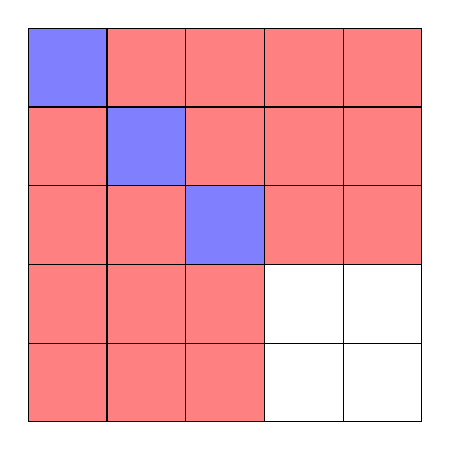
\begin{tikzpicture}
  \ColorCells{1/1/blue!50}
  \ColorCells{1/2/red!50, 1/3/red!50, 1/4/red!50, 1/5/red!50, 2/1/red!50, 3/1/red!50, 4/1/red!50, 5/1/red!50}
  \ColorCells{2/2/blue!50}
  \ColorCells{2/3/red!50, 2/4/red!50, 2/5/red!50, 3/2/red!50, 4/2/red!50, 5/2/red!50}
  \ColorCells{3/3/blue!50}
  \ColorCells{3/4/red!50, 3/5/red!50, 4/3/red!50, 5/3/red!50}
  \draw (0, 0) grid (\nx, \ny);
\end{tikzpicture}

\end{document}
